\section{Introduction}
\label{sec:testing:intro}

Manual testing is, by far, the most popular technique for
testing, but this technique is known to be error-prone as well.
As already formulated in this thesis, production systems are
usually composed of thousands of states (\emph{i.e.} sets of
conditions that exist at a given instant in time) and production
events, which makes testing time consuming.  In this context, we
propose a \emph{passive testing framework} for production systems
that is composed of two parts: a model inference engine, already
presented in Chapter \ref{sec:modelinf:prodsystems}, and a
passive testing engine that is the purpose of this chapter. Both
parts have to be fast and scalable to be used in practice.

The main idea of our proposal is that, given a running production
system, we extract knowledge and models by passively monitoring
it. Such models describe the functional behaviors of the system,
and may serve for different purposes, \emph{e.g.}, testing
another production system. The latter can be a new system roughly
comparable to the first one in terms of features, but it can also
be an updated version of the first one. Indeed, upgrades might
inadvertently introduce faults, and it could lead to severe
damages. Here, testing the updated system means detecting
potential regressions before deploying changes in production.

A \textit{passive tester} (also known as observer) aims at
checking whether a system under test \emph{conforms to} an
inferred model. It can be performed in either online or offline
mode, as defined below:

\begin{itemize}
    \item \textbf{Online testing:} sometimes called on-the-fly
        testing, it is a technique in which test case generation
        and test execution are combined into a single algorithm.
        The tester gives a verdict every time a trace incomes;

    \item \textbf{Offline testing:} it means that a set of traces
        has been collected while the system is running. Then, the
        tester gives verdicts.
\end{itemize}

We collect the traces of the system under test by reusing
\textit{Autofunk v3}'s Models generator. In offline mode, we
build a set of traces with the same level of abstraction as those
considered for inferring models. In online mode, we apply the
same process for each new incoming trace. Then, we use these
traces to check if the system under test conforms to the inferred
models. \emph{Conformance} is defined with two implementation
relations, which express precisely what the system under test
should do. The first relation corresponds to the \emph{trace
preorder} \cite{DNH84}, which is a well-known relation based upon
trace inclusion, and heavily used with passive testing.
Nevertheless, our inferred models are partials, \emph{i.e.} they
do not necessarily capture all the possible behaviors that should
happen. That is why we propose a second implementation relation,
less restrictive on the traces that should be observed from the
system under test.

Both offline and online modes are not completely unalike, they
also serve different purposes. In previous works, we used to work
with fixed sets of traces. We noticed that, by taking large trace
sets, we could build more complete models. Performing offline
passive testing allows to use such large trace sets, hence the
intuition that we should be able to validate more behaviors. Our
online passive testing approach records traces on a system under
test on-the-fly, and then check whether those traces satisfy
specifications, still generated from a system under analysis. It
enables what we call \emph{just-in-time fault detection}. Faults
can be revealed in near real-time on a running system so that
users can be notified as soon as possible.

In Section \ref{sec:testing:normal}, we introduce an extra step
of the model inference method described in Chapter
\ref{sec:modelinf:prodsystems} that is required to enable
testing. In Section \ref{sec:testing:passive}, we present both
our offline and online passive testing techniques, built on-top of
this model inference framework, respectively in Section
\ref{sec:testing:offline} and Section \ref{sec:testing:online}.
We present key results on offline passive testing in Section
\ref{sec:testing:offline:impl-exp}. Finally, we conclude on this
chapter in Section \ref{sec:testing:conclusion}.

\textbf{Publication.} This work has been partially published in
the Proceedings of the 13th International Conference on Formal
Methods and Models for Co-Design (MEMOCODE'15) \cite{7340480}.

%%%%%%%%%%%%%%%%%%%%%%%%%%%%%%%%%%%%%%%%%%%%%%%%%%%%%%%%%%%%%%%%%

\section{Extending inferred models with normalization}
\label{sec:testing:normal}

In order to perform testing, we reuse the reduced model
$R(\EuScript{S}) = \{R(\EuScript{S}_1),\dots,R(\EuScript{S}_n)\}$
inferred with \textit{Autofunk} that we \textit{normalize} to get
rid of some runtime-dependent information.  Indeed, both models
$\EuScript{S}$ and $R(\EuScript{S})$ include parameters that are
dependent to the products being manufactured.  That is a
consequence of generating models that describe behaviors of a
continuous stream of products that are strictly identified,
\emph{i.e.} for each action in a given sequence, we have the
assignment $(pid := val)$ (for the record, $pid$ stands for
\emph{product identifier}).  Here, we normalize these models
before using them for testing.  The resulting models are denoted
by $\EuScript{S}^{N}$ and $R(\EuScript{S}^{N})$.

We remove the assignments relative to product identifiers and
time stamps. Furthermore, we label all the final locations with
"Pass". We flag these locations as \emph{verdict locations}, and
gather them in the set $Pass \subseteq L_{\EuScript{S_i}^{N}}$.
Both $\EuScript{S}^{N}$ and $R(\EuScript{S}^{N})$ represent more
generic models, \emph{i.e.}  they express \textit{some possible
behaviors that should happen}. These behaviors are represented by
the traces $Traces_{Pass} (\EuScript{S}^{N})=\displaystyle
\bigcup_{1 \leq i \leq n} Traces_{Pass}
(\EuScript{S}_i^{N})=Traces_{Pass} (R(\EuScript{S}^{N}))$. We
refer to these traces as \textit{pass traces}. We call the other
traces \textit{possibly fail traces}.

%%%%%%%%%%%%%%%%%%%%%%%%%%%%%%%%%%%%%%%%%%%%%%%%%%%%%%%%%%%%%%%%%

\section{Passive testing with \textit{Autofunk}}
\label{sec:testing:passive}

We consider both models $\EuScript{S}^{N}$ and
$R(\EuScript{S}^{N})$ of a system under analysis $\mathit{Sua}$,
generated by our inference-based model generation framework, as
\emph{reference models}. In this section, we present the second
part of our framework, dedicated to the passive testing of a
system under test $\mathit{Sut}$.

Figure \ref{fig:passive-autofunk} depicts the architecture of our
passive testing technique. In offline mode, a set of production
events has been collected beforehand from $\mathit{Sut}$ in the
same way as for $\mathit{Sua}$. These events are grouped into
traces to form the trace set $Traces({Sut})$, and then filtered
to obtain a set of complete traces denoted by $CTraces({Sut})$
(cf.
\crossref{sec:modelinf:prodsystems}{sec:modelinf:prodsystems:better-segmentation}).
In online mode (not represented on the figure), we do not have
traces but rather filtered valued events of $\mathit{Sut}$ coming
on-the-fly. Finally, we perform passive testing to \emph{check}
if $\mathit{Sut}$ conforms to $\EuScript{S}^{N}$.

\begin{figure}[h]
    \begin{center}
        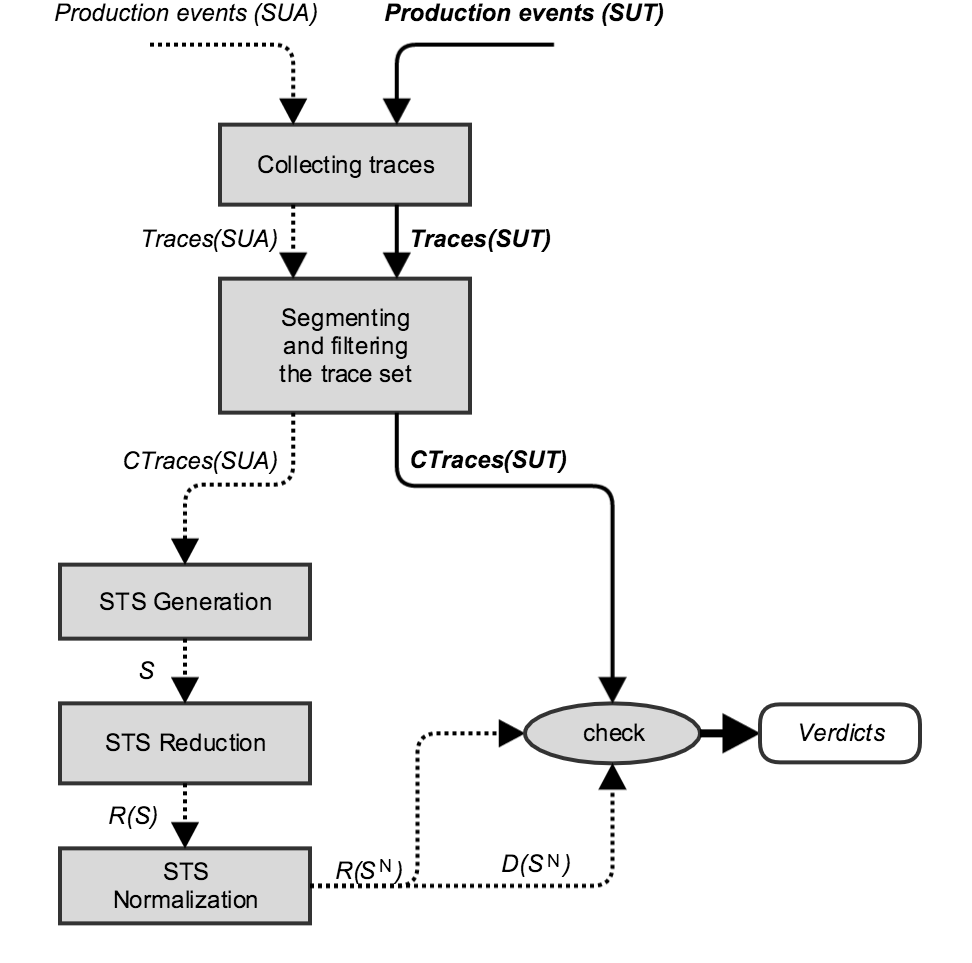
\includegraphics[width=1.0\linewidth]{figures/passive_autofunk.png}
    \end{center}

    \caption{The architecture of \textit{Autofunk v3} with the
    passive testing extension. While the previous
    \textit{Autofunk}'s architecture has been kept, there are
    two new modules: "STS Normalization" and "check",
    representing the passive conformance testing part.}
    \label{fig:passive-autofunk}
\end{figure}

Our industrial partner wishes to check whether every complete
execution trace of $\mathit{Sut}$ matches a behavior captured by
$\EuScript{S}^{N}$. In this case, the test verdict must reflect a
successful result. On the contrary, if an execution of
$\mathit{Sut}$ is not captured by $\EuScript{S}^{N}$, one cannot
conclude that $\mathit{Sut}$ is faulty because $\EuScript{S}^{N}$
is a partial model, and it does not necessarily includes all the
correct behaviors. Below, we formalize theses verdict notions
with two implementation relations. Such relations between models
can only be written by assuming the following \emph{test
assumption}: the black-box system $\mathit{Sut}$ can be described
by a model, here with a Labeled Transition System as defined in
\crossref{sec:related:testing}{sec:definitions:lts}. We also
denote this model by $\mathit{Sut}$.

The first implementation relation, denoted by $\leq_{ct}$, refers
to the trace preorder relation
\cite{DNH84,vaandrager1991relationship} (cf. Example
\ref{example:trace_preorder} on page
\pageref{example:trace_preorder}).
It aims at checking whether all the complete execution traces of
$\mathit{Sut}$ are pass traces of
$\EuScript{S}^{N}=\{\EuScript{S}_1^{N},\dots,\EuScript{S}_n^{N}\}$.
The first implementation relation can be written with the
following definition:

\begin{definition}[The $\leq_{ct}$ implementation relation]
\label{rel:impl1}

Let $\EuScript{S}^{N}$ be an inferred model of $\mathit{Sua}$, and
$\mathit{Sut}$ be the system under test. When $\mathit{Sut}$
produces complete traces also captured by $\EuScript{S}^{N}$, we
write: ${Sut} \leq_{ct} \EuScript{S}^{N} =_{def} CTraces({Sut})
\subseteq  Traces_{Pass}(\EuScript{S}^{N})$.
\end{definition}

Pragmatically, the reduced model $R(\EuScript{S}^{N})$ sounds
more convenient for passively testing $\mathit{Sut}$ since it is
strongly reduced in terms of size compared to $\EuScript{S}^{N}$.
The test relation can also be written as below since both models
$\EuScript{S}^{N}$ and $R(\EuScript{S}^{N})$ are trace equivalent:

\begin{proposition}
\label{rel:impl12}
${Sut} \leq_{ct} \EuScript{S}^{N} \text{ if and only if } CTraces({Sut})
\subseteq  Traces_{Pass}(R(\EuScript{S}^{N}))$.
\end{proposition}

As stated previously, the inferred model $\EuScript{S}^{N}$ of
$\mathit{Sua}$ is partial, and might not capture all the
behaviors that should happen on $\mathit{Sut}$. Consequently,
our partner wants a weaker implementation relation that is less
restrictive on the traces that should be observed from
$\mathit{Sut}$.  In other words, this second relation aims to check
that, for every complete trace $t=a_1(\alpha_1)...a_m(\alpha_m)$
of $\mathit{Sut}$, we also have a set of traces of
$Traces_{Pass}(\EuScript{S}^{N})$ having the same sequence of
symbols such that every variable assignment $\alpha_j(x)_{(1 \leq
j \leq m)}$ of $t$ is found in one of the traces of
$Traces_{Pass}(\EuScript{S}^{N})$ with the same symbol $a_j$.
If we take back the example of Figure \ref{fig:firstmodel}, the
trace $t=(17011(nsys:=1,nsec:=8,point:=1,pid:=1)\text{ }
17021(nsys:=1,nsec:=8,point:=4,tpoint:=9,pid:=1)$ is not a pass trace
of $\EuScript{S}^{N}$ because this trace cannot be extracted from
one of the paths of the STS of Figure \ref{fig:firstmodel}, on
account of the variables $point$ and $tpoint$, which do not take
the expected values. Nonetheless, both variables are assigned
with $point:=4,tpoint:=9$ in the second path. This is interesting
as it indicates that such values may be correct since they are
actually used in a similar action in a similar path. Here, the
second implementation relation aims at expressing that this trace
$t$ captures a correct behavior as well.

\TODO{first model?}

% \begin{comment}
% This second implementation relation, denoted with $\leq_{mct}$, is written
% with the classes of equivalent paths $[b]$, found in a STS of
% $\EuScript{S}^{N}=\{\EuScript{S}_1^{N},...,\EuScript{S}_n^{N}\}$.
% Indeed, an equivalent class $[b]$ of $\EuScript{S}_i^{N}$ gathers
% STS paths having the same sequence of labels but with
% different guards. The definition of $\leq_{mct}$, given below,
% means that for a trace $t$, an equivalence class $[b]$ must be
% found such that for every valued action $a_j(\alpha_j)$, each
% variable assignment $\alpha_j(x)$ with $x$ a variable, must
% satisfies at least on the guards $G_{j1},...,G_{jk}$ found on
% the transitions labeled with $a_j(p_j)$:
%
% \begin{proposition}
%     Let $\mathit{Sua}$ be the system under analysis,
%     $\EuScript{S}^{N}=\{\EuScript{S}_1^{N},\dots,\EuScript{S}_n^{N}\}$ be its inferred model and $\mathit{Sut}$ be the system under test.
%     We denote ${Sut} \leq_{mct} \EuScript{S}^{N} =_{def} \forall t=
%     a_1(\alpha_1)...a_m(\alpha_m) \in CTraces({Sut}), \exists
%     \EuScript{S}_i^{N} \text{ and } [b]=\{l0_{\EuScript{S}_i^{N}} \xRightarrow{(a_1(p_1),G_{1o}),...,(a_m(p_m),G_{mo})}l_{mo} (1 \leq o \leq k) \}$ such that $\forall \alpha_j(x) (1 \leq j \leq m), \alpha_j(x) \models G_{j1} \vee ... \vee  G_{jk}$ and $l_{mo} \in Pass$.
% \end{proposition}
%
% This relation can be reformulated with the reduced model
% $R(\EuScript{S}^{N})=\{R(\EuScript{S}_1^{N}),\dots,R(\EuScript{S}_n^{N})\}$,
% which reduces the equivalence classes $[b]$ into one STS path.
% Given a trace $a_1(\alpha_1)...a_m(\alpha_m)$, the relation can
% be now written with matrices of guards: for every valued action
% $a_j(\alpha_j)$, each variable assignment $\alpha_j(x)$ must now
% satisfies one of the guards of the matrix line $j$ in
% $M_{[b]}[j,*]$.  If, we take back the trace example
% $t=(17011(nsys=1,nsec=8,point=1,pid=1)\text{ }
% 17021(nsys=1,nsec=8,point=4,tpoint=9,pid=1)$, and the STS of
% Figure \ref{fig:reduced-model}, the assignment $point=4$, which
% is given with the second valued action of $t$, satisfies one of
% the guards of the second line of the matrix $M_{[b]}$.
% \end{comment}

This implementation relation, denoted by $\leq_{mct}$, is
written with:

\begin{definition}[The $\leq_{mct}$ implementation relation]
	\label{impl21}
	 Let $\EuScript{S}^{N}$ be an inferred model of $\mathit{Sua}$ and
	 $\mathit{Sut}$ be the system under test.

     We denote by ${Sut} \leq_{mct} \EuScript{S}^{N} =_{def} \forall
     t= a_1(\alpha_1) \dots a_m(\alpha_m) \in CTraces({Sut}),
     \forall \alpha_j(x)_{(1 \leq j \leq m)},\\ \exists
     \EuScript{S}_i^{N} \in \EuScript{S}^{N} \text{ and } t'\in
     Traces_{Pass}(\EuScript{S}_i^{N})$ such that
     $t'=a_1(\alpha_1')...a_m(\alpha_m')$ \text{ and }
     $\alpha_j'(x)=\alpha_j(x)$.
\end{definition}

In the following, we rewrite this relation in an equivalent but
simpler form. According to the above definition, the successive
symbols and variable assignments of a trace $t \in
CTraces({Sut})$ must be found into several traces of
$Traces_{Pass}(\EuScript{S}_i^{N})$, which have the same sequence
of symbols $a_1...a_m$ as the trace $t$. The reduced model
$R(\EuScript{S}_i^{N})$ was previously constructed to capture
all these traces in $Traces_{Pass}(\EuScript{S}_i^{N})$, having
the same sequence of symbols. Indeed, given a STS
$\EuScript{S}_i^{N}$, all the STS paths of $\EuScript{S}_i^{N}$,
which have the same sequence of symbols labeled on the
transitions, are compacted into one STS path $b$ in
$R(\EuScript{S}_i^{N})$ whose transition guards are stored into a
matrix $M_{[b]}$.

If, we take back the trace example
$t=(17011(nsys:=1,nsec:=8,point:=1,pid:=1)\text{ }
17021(nsys:=1,nsec:=8,point:=4,tpoint:=9,pid:=1))$, and the STS of
Figure \ref{fig:reduced-model}, $t$ is a pass trace with respect
to $\leq_{mct}$ because each assignment $\alpha_j(x)$ satisfies
at least one guard of the matrix line $j$. For instance, the
assignment $point:=4$, which is given with the second valued
action of $t$, satisfies one of the guards of the second line of
the matrix $M_{[b]}$.

Given a trace $a_1(\alpha_1) \dots a_m(\alpha_m) \in CTraces({Sut})$
and a STS path $b$ of $R(\EuScript{S}_i^{N})$ having the same
sequence of symbols $a_1 \dots a_m$, the relation can be now
formulated as follows: for every valued action $a_j(\alpha_j)$,
each variable assignment $\alpha_j(x)$ must satisfies at least
one of the guards of the matrix line $j$ in $M_{[b]}[j,*]$.

The implementation relation $\leq_{mct}$ can then be written with:

\begin{proposition}
	${Sut} \leq_{mct} \EuScript{S}^{N} \text{ if and only if } \forall t=
	a_1(\alpha_1) \dots a_m(\alpha_m) \in CTraces({Sut}), \exists
	R(\EuScript{S}_i^{N}) \in R(\EuScript{S}^{N)} \text{ and }
	b=l0_{R(\EuScript{S}_i^{N})} \xRightarrow{(a_1(p_1),M_{[b]}[1,c_{[b]}]),\dots,(a_j(p_j),M_{[b]}[j,c_{[b]}])} l_m$ with $(1 \leq c_{[b]} \leq k)$ such that $\forall \alpha_j(x) (1 \leq j \leq m), \alpha_j(x) \models M_{[b]}[j,1] \vee \dots \vee  M_{[b]}[j,k]$ and $l_m \in Pass$.
\end{proposition}

% \begin{comment}
% This second implementation relation, denoted with $\leq_{mct}$, can be written with the reduced model
% $R(\EuScript{S}^{N})=\{R(\EuScript{S}_1^{N}),\dots,R(\EuScript{S}_n^{N})\}$. Indeed, given a STS $\EuScript{S}_i^{N}$, all the STS paths of$\EuScript{S}_i^{N}$, which have the same sequence of symbols labeled on the transitions, are compacted into one STS path $b$ in $R(\EuScript{S}_i^{N})$ whose transition guards are stored into a matrix $M_{[b]}$. Given a trace $a_1(\alpha_1)...a_m(\alpha_m) \in CTraces({Sut})$ and a STS path $b$ of $R(\EuScript{S}_i^{N})$ having the same sequence of symbols $a_1...a_m$, the relation can
% be now formulated as follows: for every valued action
% $a_j(\alpha_j)$, each variable assignment $\alpha_j(x)$ must
% satisfies at least one of the guards of the matrix line $j$ in
% $M_{[b]}[j,*]$.
%
%
%
%
% If, we take back the trace example
% $t=(17011(nsys=1,nsec=8,point=1,pid=1)\text{ }
% 17021(nsys=1,nsec=8,point=4,tpoint=9,pid=1)$, and the STS of
% Figure \ref{fig:reduced-model}, the assignment $point=4$, which
% is given with the second valued action of $t$, satisfies one of
% the guards of the second line of the matrix $M_{[b]}$. Hence, $t$ represents a correct behaviour w.r.t. the STS of
% Figure \ref{fig:reduced-model}.
%
% \begin{definition}
%     ${Sut} \leq_{mct} \EuScript{S}^{N} \text{ iff } \forall t=
%     a_1(\alpha_1)...a_1(\alpha_m),\\ \exists
%     R(\EuScript{S}_i^{N}) \text{ and } l0_{R(\EuScript{S}_i^{N})} \xRightarrow{(a_1(p_1),G_{1}),...,(a_m(p_m),G_{m})} l_m$ such that $\forall \alpha_j(x) (1 \leq j \leq m), \alpha_j(x) \models M_{[b]}[j,1] \vee ... \vee  M_{[b]}[j,k]$ and $l_m \in Pass$.
% \end{definition}
% \end{comment}

The disjunction of guards $M_{[b]}[j,1] \vee \dots \vee
M_{[b]}[j,k]$, found in the matrix $M_{[b]}$, could be simplified
by gathering all the equalities $x==val$ together with
disjunctions for every variable $x$ that belongs to the parameter
set $p_j$. Such equalities can be extracted with the projection
operator \textit{proj} (see Definition \ref{def:sts}). We obtain
one guard of the form $\bigwedge_{x \in p_j}(x==val_1 \vee \dots
\vee x==val_k)$. The STS $D(\EuScript{S}_i^{N})$, derived from
$R(\EuScript{S}_i^{N})$, is constructed with this simplification
of guards:

%all the variable assignments found in the guards
%$M_{[b]}[j,1],..., M_{[b]}[j,k]$ can be collected with the
%projection operator $proj_{x}(G)$.

%It is then possible to create
%vectors of guards from the matrices in $R(\EuScript{S}_i)^{G}$ in
%order to express that a trace $t$ can still comply with the
%behaviours found in $R(\EuScript{S}_i)^{G}$, even if it does not
%strictly satisfy all guards of a single branch (\emph{i.e.} the same
%column in the matrices), but rather the disjunction of the guards
%belonging to the matrices of this branch.

\begin{definition}[Derived STS $D(\EuScript{S}_i^{N})$]
    Let
    $R(\EuScript{S}_i^{N})=<L_R,l0_R,V_R,V0_R,I_R,\Lambda_R,\rightarrow_R>$
    be a STS of $R(\EuScript{S}^{N})$. We denote by $D(\EuScript{S}_i^{N})$ the STS $ <L_D,l0_D,V_D,V0_D,I_D,\Lambda_D,\rightarrow_D>$ derived from $R(\EuScript{S}_i^{N})$ such that:
\begin{itemize}
    \item $L_D=L_{R}, l0_D=l0_{R}, I_D=I_{R},
        \Lambda_D=\Lambda_{R}$;
    \item $V_D, V0_D$ and $\rightarrow_D$ are given by the following inference rule:

				$\frac{
					\begin{matrix}
					b=l0_{R}
					\xRightarrow{(a_1(p_1),M_{[b]}[1,c_{[b]}])\dots (a_m(p_m),M_{[b]}[m,c_{[b]}]}_{\rightarrow_{R}}
					l_{m},
					(1 \leq c_{[b]} \leq k) \text{ in } V0_{R}
					\end{matrix}
				}
				{
					\begin{matrix}
					l0_D
					\xRightarrow{(a_1(p_1),M_b[1])\dots (a_m(p_m),M_b[m])}_{\rightarrow_D}
					l_m\\
					V_D=V0_D \wedge M_b, M_b[j, 1]_{(1\leq j \leq m)} =\\
					 \displaystyle \bigwedge_{x \in p_j} ( proj_x(M_{[b]}[j, 1]) \vee \dots \vee proj_x(M_{[b]}[j, k]))


					%\bigvee_{1 \leq k \leq k} proj_x ((M_{[b]}[j, k])

					\end{matrix}
				}$
  \end{itemize}

    $D(\EuScript{S}^{N})$ denotes the model $\{D(\EuScript{S}_1^{N}),\dots,D(\EuScript{S}_n^{N}) \}$.
\end{definition}


The second implementation relation $\leq_{mct}$ can now be
expressed by:

\begin{proposition}
    ${Sut} \leq_{mct} \EuScript{S}^{N} \text{ if and only if }\forall t=
    a_1(\alpha_1) \dots a_m(\alpha_m) \in CTraces({Sut}), \exists
    D(\EuScript{S}_i^{N}) \in D(\EuScript{S}^{N}) \text{ and }
    l0_{D(\EuScript{S}_i^{N})}
    \xRightarrow{(a_1(p_1),G_{1}),\dots,(a_m(p_m),G_{m})} l_m
    \text{ such that } \forall \alpha_j (1 \leq j \leq m),
    \alpha_j \models G_{j}$ and $l_m \in Pass$.
\end{proposition}


$\leq_{cmt}$ now means that a trace of $\mathit{Sut}$ must also
be a pass trace of the model
$D(\EuScript{S}^{N})=(D(\EuScript{S}_1^{N}),\dots,D(\EuScript{S}_n^{N}))$.
Furthermore, this notion of trace inclusion can be formulated
with the first implementation relation $\leq_{ct}$ as follows:

\begin{proposition}
	\label{rel:impl2}
${Sut} \leq_{mct} \EuScript{S}^{N} \text{ if and only if } CTraces({Sut})\subseteq Traces_{Pass}(D(\EuScript{S}^{N}))$

${Sut} \leq_{mct} \EuScript{S}^{N}\Leftrightarrow {Sut} \leq_{ct} D(\EuScript{S}^{N})$

\end{proposition}

The implementation relation $\leq_{mct}$ is now expressed with
the first relation $\leq_{ct}$, which implies that our passive
testing algorithms shall be the same for both relations but shall
take different reference models.
In the next section, we introduce an offline passive testing
algorithm that uses these two implementation relations.
